\section{CMS Track Trigger System Overview}

\subsection{Overview}

\noindent The extremely high luminosities foreseen at the HL-LHC pose many unique challenges to a possible track trigger system based on silicon detectors, this is especially true at Level 1. As mentioned earlier, the input data bandwidth is expected at about 50 Tbps and the total Level 1 trigger latency has to stay within about 10 microseconds, with only a few microseconds or so available for track processing. This includes data transfer, trigger tower formation, pattern recognition, track fitting and any necessary further processing such as, for example, jet vertexing. 

\noindent Many unique challenges must be faced at the different stages of the processing chain: first, data need to be transferred out of the tracker at the necessary speed, stubs from thousands of silicon modules must be formatted, organized into $\eta$/$\phi$ trigger towers, duplicated and shared across tower boundaries as needed, then we need to perform pattern recognition and track fitting, and finally process all the tracks reconstructed by the previous stages to form an intelligent trigger decision. A coherent system design for a Level-1 track trigger will include all these aspects.

\noindent In this document we will make the working assumption that there will be a total of 15K detector modules/fibers, each fiber with 3.25 Gbps payload (about 50Tbps total raw bandwidth). The detector will be partitioned into 48 trigger towers, six in $\eta$ and eight in $\phi$. Each trigger tower will therefore handle 312 modules/fibers on average. The cabling of the modules will need to be optimized for trigger requirements. For simplicity, we will assume that the FEDs will receive the fibers from the modules and pass the relevant data to the track trigger system even though the architecture could allow the FED to reside in the same ATCA shelf as the track trigger data input boards on dedicated AMC ATCA carrier boards. The focus of this document is the Vertical Slice Demonstration System, not the DAQ readout, so FED details are not discussed here (they belong to TK-DAQ). The FED interface will need to be defined for demonstration purpose, even though the actual FEDs do not have to be involved in the demonstration.

\subsection{Tracker-Trigger interface}

\subsubsection{Block Synchronous Data Transfer scheme }

\noindent The found stubs are sent from the modules using a block synchronous data transfer scheme, which tolerates random occupancy fluctuations while bonding latency. Current plan is to have the data from 8 consecutive beam crossings as one block. The front-end designers are still investigating different format variants for robustness against rate fluctuations, ease of implementation, impact on power consumption etc. While choosing the 8 crossings scheme as our current working assumption, our strategy is to design the downstream components to be flexible enough to handle different possible formats.

\subsubsection{Relevant design studies}

\noindent There are many studies we still need to do to understand the system requirements much beyond data transfer. Will make a list here soon (such as actual stub distribution at module output level, zero suppression scheme and data formatting, at input to the pattern recognition engine after the block transfer, and what's the maximal stub occupancy the system should handle etc).

\subsection{Track Trigger System Architecture}

\subsubsection{Tracker geometry and Trigger Towers }

\noindent Detailed studies have been done for the BE tracker geometry with different trigger tower partitions, and the 6 (in eta) x 8 (in phi) = 48 trigger tower partition has been chosen as the default baseline configuration (see Figures~\ref{fig:SecDef_RZ} \& \ref{fig:SecDef_XY}).

\begin{figure}[ht!]
\centering
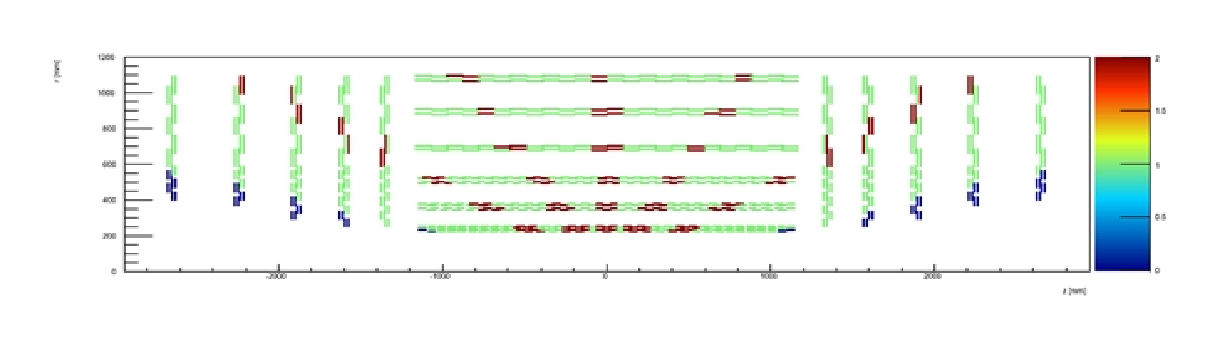
\includegraphics[width=0.8\columnwidth]{Plots/SecDef_RZ.eps}
\caption{Six sectors in $\eta$. Note that the symmetry around $\eta=0$ will provide for easier cable grouping}
\label{fig:SecDef_RZ}
\end{figure}
\begin{figure}[ht!]
\centering
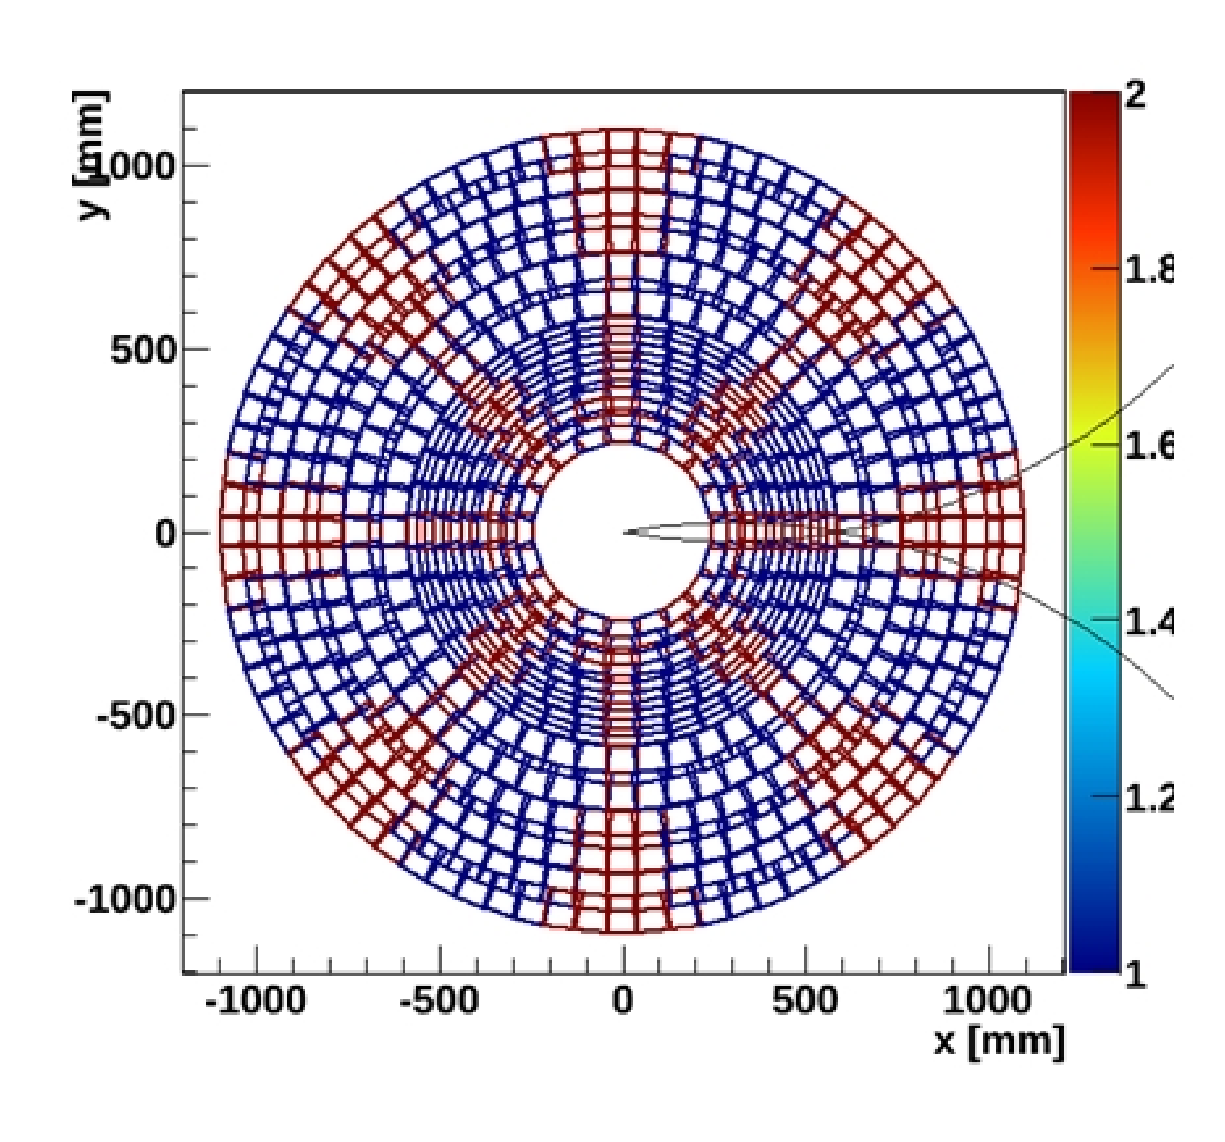
\includegraphics[width=0.4\columnwidth]{Plots/SecDef_XY.eps}
\caption{Eight sectors in phi}
\label{fig:SecDef_XY}
\end{figure}

\noindent Stubs from the 15K silicon modules must be delivered each one to the correct trigger towers. Due to the finite size of the beam's luminous region in z and the finite pT curvature of charged particles in the magnetic field, some of the stubs, coming from the neighborhood of some tower boundary, must be delivered to multiple towers to avoid efficiency gaps.  Detailed studies have been performed on data sharing assuming the default 48 tower partition, a minimum Pt of 2GeV and track origin smearing in z +- 7cm. Figure~\ref{fig:SecDef_N} shows the distribution of the number of trigger towers stubs from a given module should be delivered to in these conditions. When a stub is in the middle of the trigger tower, it will have to be delivered to only one tower (to the native trigger tower). When a stub is at the boundary in phi or eta (but not both), it will have to be delivered to two towers. If a stub is at both the boundaries in eta and phi, it will have to be delivered to four towers. Note that four towers is the absolute maximum number of towers any stub must be delivered to. 

\begin{figure}[ht!]
\centering
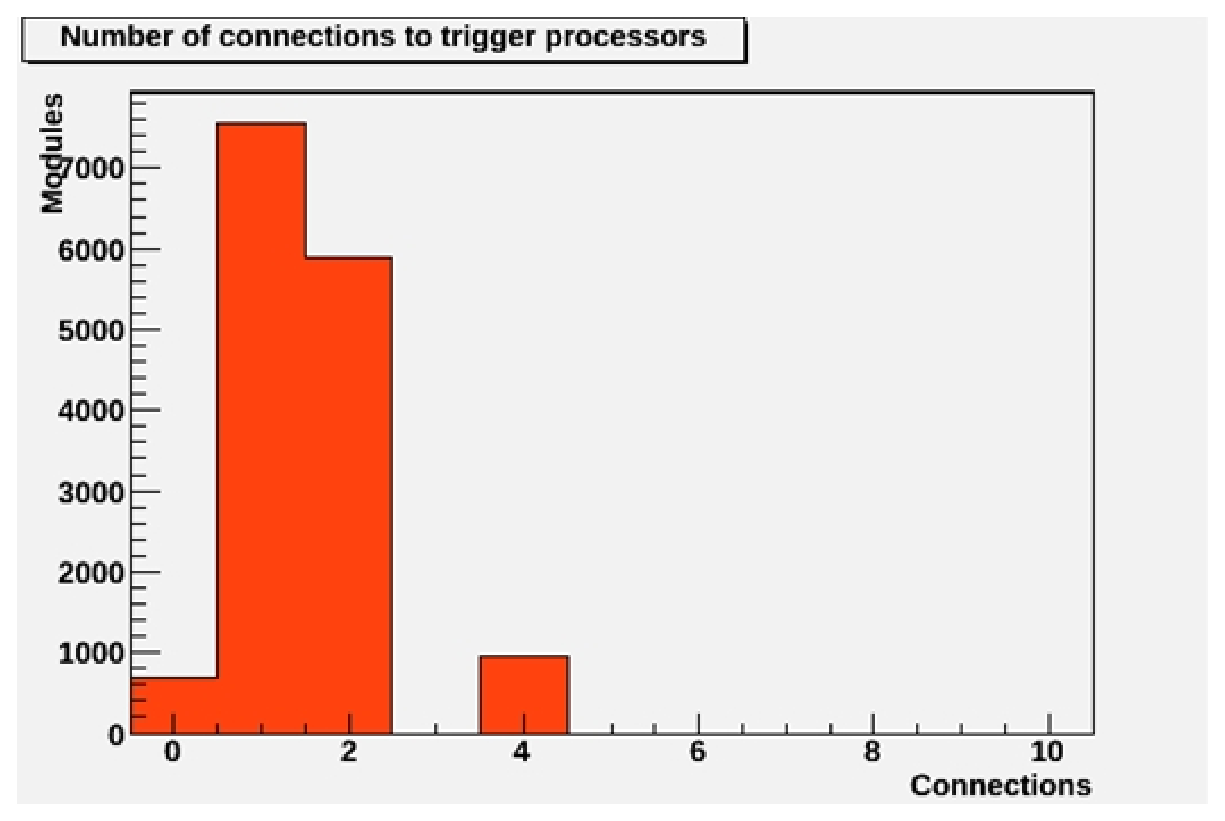
\includegraphics[width=0.45\columnwidth]{Plots/SecDef_N.eps}
\caption{Distribution of the number of trigger towers each module needs to be connected to. Entries at zero are from modules that do not participate in triggering}
\label{fig:SecDef_N}
\end{figure}

\subsubsection{Formation of Trigger Towers}

\noindent The phase II tracker is being designed and optimized keeping in mind the trigger requirements. The resulting formation of the 48 Trigger towers is shown in Figure~\ref{fig:TT_config}, where the lines indicate all needed interconnections among the trigger towers. The nice feature of this arrangement is that any given trigger tower only needs to be connected and share stubs with its immediate eight neighbors. This inter-connection structure will be used as the foundation of the proposed trigger system architecture. Detailed studies have shown that this architecture is not sensitive to the variations of minimum Pt threshold, nor to the track origin in z (studied up to +- 15 cm).

\begin{figure}[ht!]
\centering
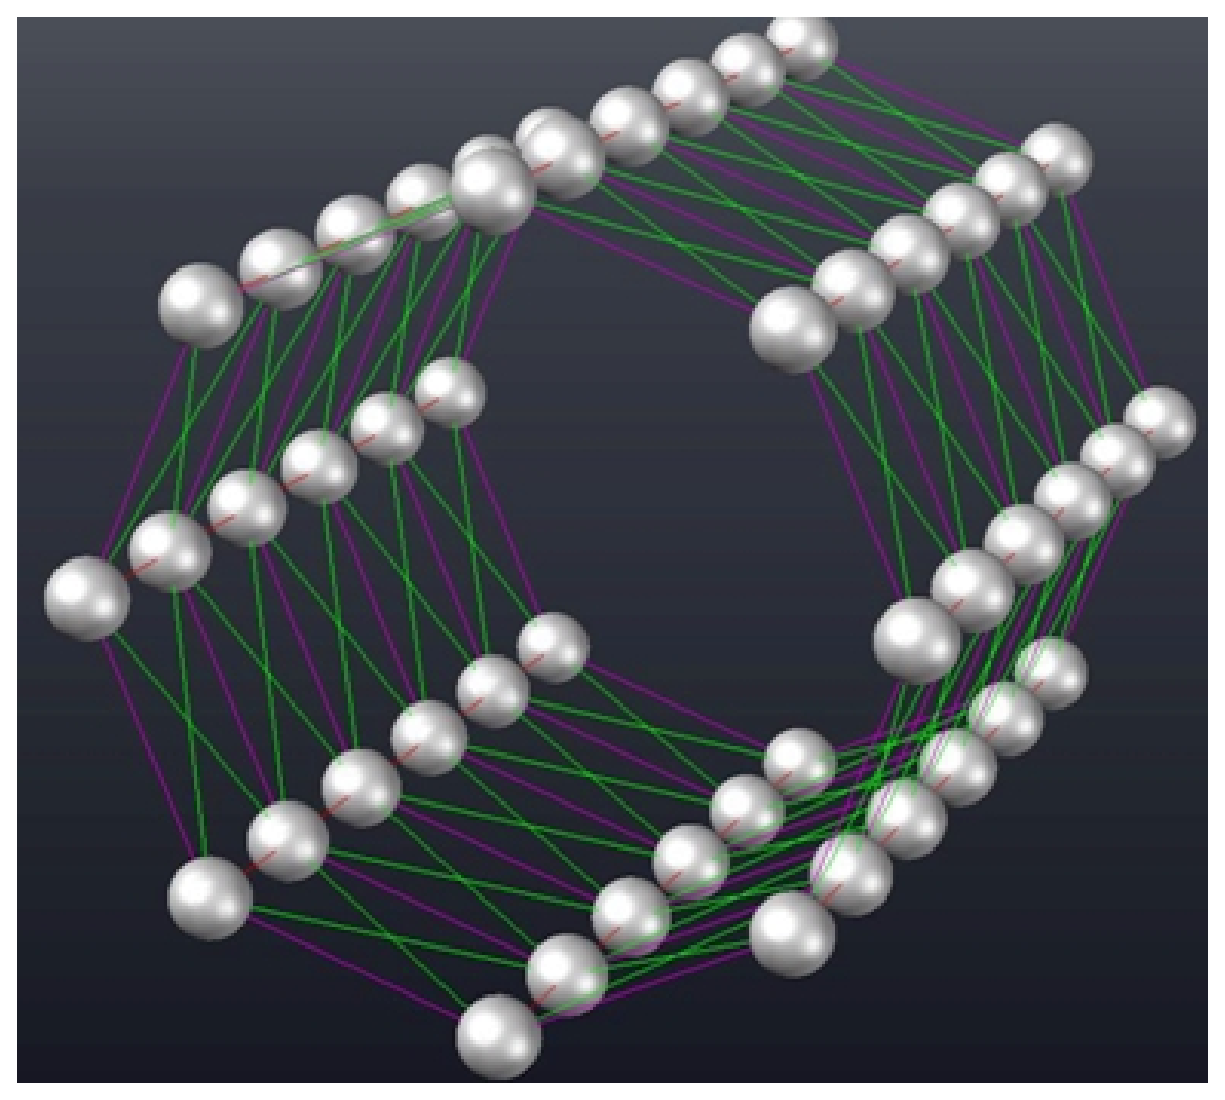
\includegraphics[width=0.6\columnwidth]{Plots/TT_config.eps}
\caption{Conceptual view of the proposed CMS phase II L1 tracking trigger towers.  The formation is organized as 48 trigger towers (6 $\eta$ x 8 $\phi$).  Because the phase II tracker is being designed for tracking trigger purposes, it is possible to arrange the towers in such a way that data sharing only requires communication with immediate neighbor towers.  Each node in this diagram represents a trigger tower processor engine.  Within each processor engine crate the full mesh backplane is used for time multiplexing of the incoming data, while the data sharing between towers is handled with inter-crate fiber links.}
\label{fig:TT_config}
\end{figure}

\noindent Our hardware design process followed a bottom up approach whereby we studied various track trigger architectures by first studying the trigger tower formation and data sharing needs. Please note that this track trigger architecture for CMS L1 is rather different from that of FTK for Atlas L2. In the case of FTK, the Atlas tracker was not designed for track trigger purpose, and the cabling was optimized for readout not for trigger. The data sharing between processing nodes is largely asymmetric and highly dependent upon upstream cabling and detector geometry. FTK chooses 64 trigger towers (16 in $\phi$ and 4 in $\eta$), and the inter-connections among the trigger towers are much more complex as a result, see Figure~\ref{fig:TT_config_ATLAS} for comparison. 

\begin{figure}[ht!]
\centering
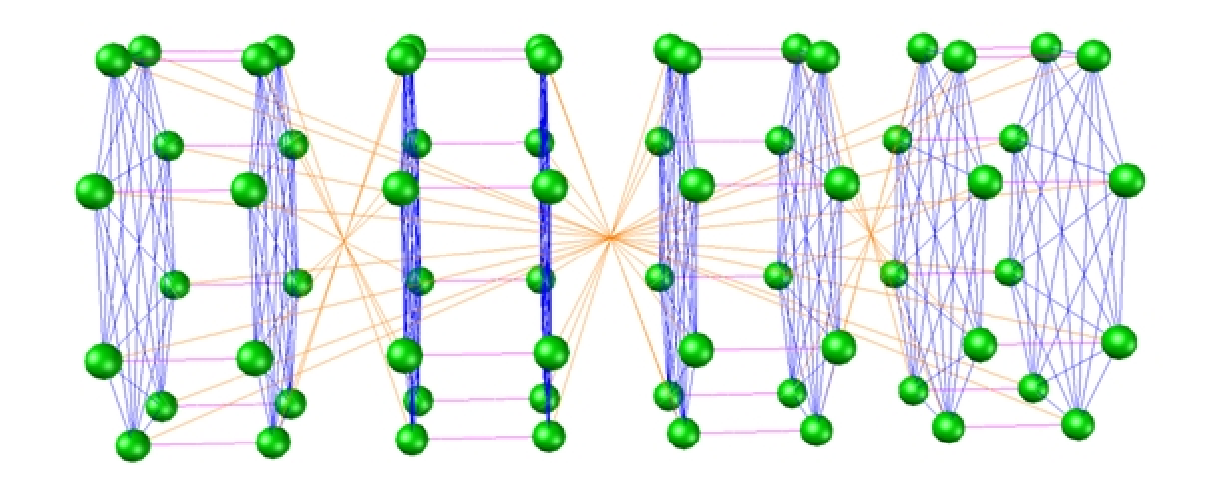
\includegraphics[width=0.7\columnwidth]{Plots/TT_config_ATLAS.eps}
\caption{Conceptual view of the ATLAS L2 Fast Tracker (FTK) Data Formatter architecture.  The FTK system is organized as 64 trigger towers (4 $\eta$ x 16 $\phi$), represented here by the green nodes.  Because the existing silicon tracker was not designed for triggering, the data sharing among trigger towers is complex as indicated by the lines connecting the nodes.  This requires the use of a full mesh backplane (shown in blue) for data sharing.  Orange lines represent inter-crate links.}
\label{fig:TT_config_ATLAS}
\end{figure}

\subsubsection{System architecture}

\noindent The tower processor platform must support large numbers of fiber transceivers, which are used for receiving input links and sharing data between neighboring towers.  A flexible, high bandwidth backplane is also required to quickly transfer data between boards.  The boards should be large enough to support AM chip arrays and fiber connections.  Given these requirements, we conclude that a full mesh 14 slot ATCA shelf is a natural fit for the tower processor.  Therefore we propose a L1 Tracking Trigger system comprised of 49 ATCA shelves, one shelf per trigger tower with an additional shelf acting as a second stage processor, as shown on Fig.~\ref{fig:System_1}. Connections between tower processor shelves are limited to eight nearest neighbors.

\begin{figure}[ht!]
\centering
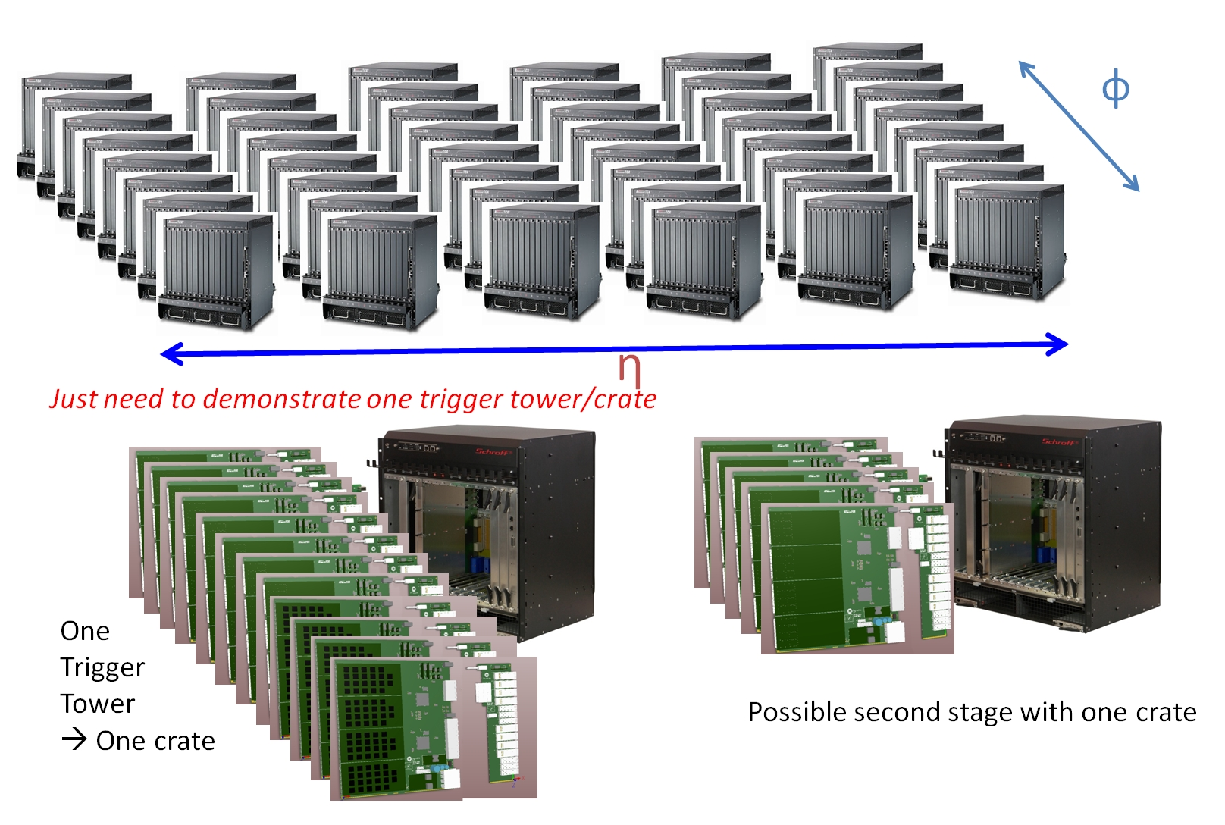
\includegraphics[width=0.7\columnwidth]{Plots/System_1.eps}
\caption{Possible system configuration with today's technilogy (smaller in the future)}
\label{fig:System_1}
\end{figure}

\noindent The fundamental baseline processing element is a pattern recognition mezzanine (PRM) card which consists of an AM chip array, where coarse roads are found, and an FPGA which performs the final track fitting. Time multiplexed data transfers into several parallel PRMs are required to reduce bandwidth to manageable levels.

\noindent An ATCA shelf is typically an air-cooled 13U rack mounted chassis consisting of 14 slots.  The first two slots are reserved for Ethernet switch blades.  Switch blades may include a fast CPU and are often used for controls and other system functions.  The remaining 12 slots are used for processor or payload blades.  In a full mesh ATCA backplane each pair of slots is directly connected with a multi-lane bidirectional serial channel capable of supporting sustained 40 Gbps data transfers.  A modern "40G" full mesh ATCA shelf has a total aggregate bandwidth of over 7 Tbps, not including external I/O.

\begin{figure}[ht!]
\centering
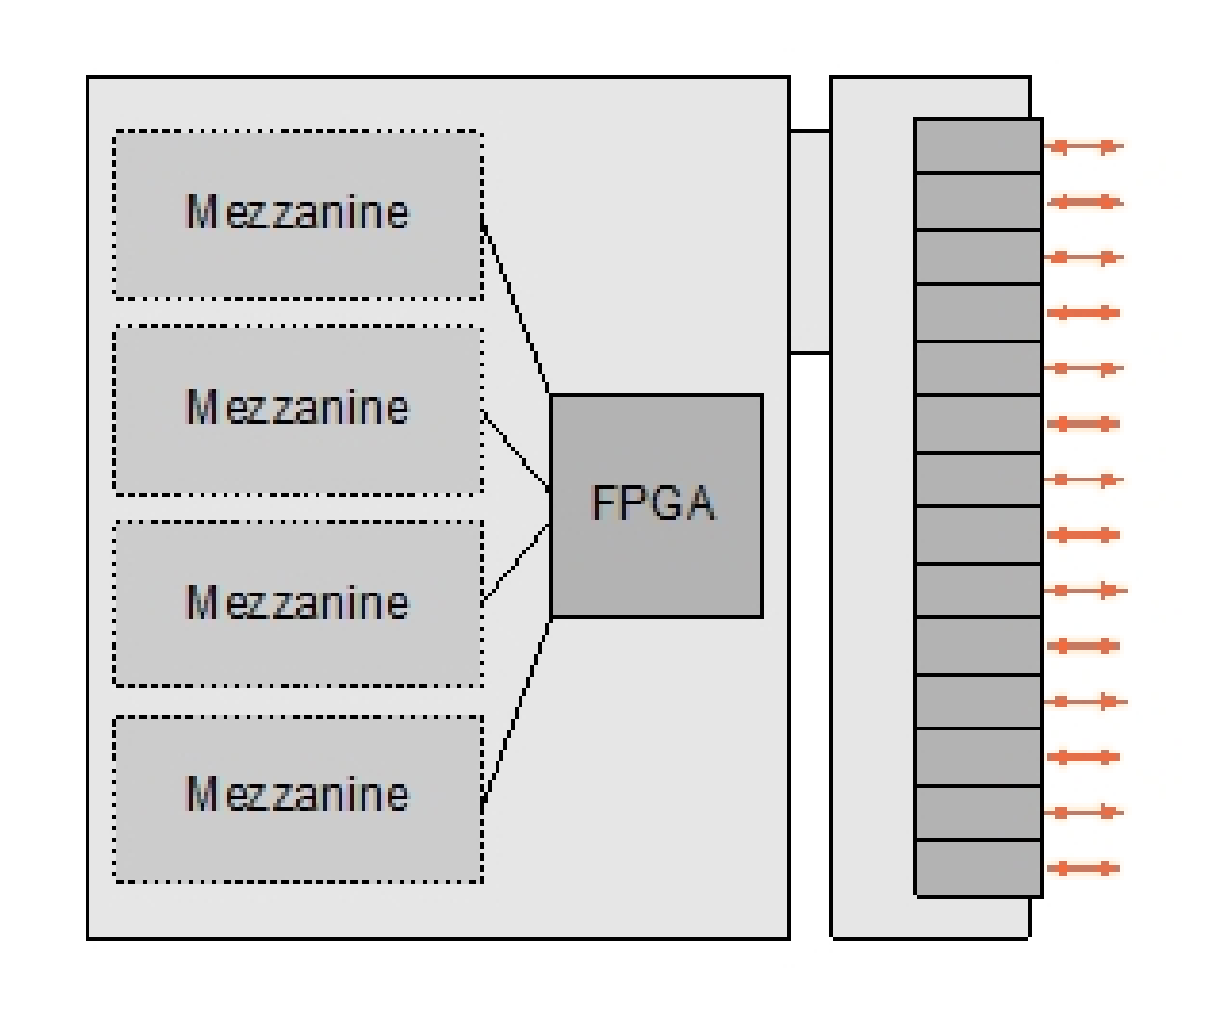
\includegraphics[width=0.45\columnwidth]{Plots/ProcBlade.eps}
\caption{Generic processor blade}
\label{fig:ProcBlade}
\end{figure}

\noindent The generic processor blade is shown in Figure~\ref{fig:ProcBlade}.  The front board measures 8U x 280mm and is designed around a single FPGA.  This FPGA connects directly to the full mesh backplane fabric, mezzanine cards, and fiber transceivers located on a rear transition module (RTM).  For the most part communication channels are high speed serial point to point links and are directly supported by SERDES transceivers in the FPGA.   

\subsubsection{Architecture/System Flexibility (optional reading)}

\noindent A major advantage of the full mesh backplane is that it effectively blurs the distinction between boards, thus enabling system architects to experiment with different shelf configurations.  Components can be roughly categorized into functional blocks such as input link receivers, AM array processors, inter-crate gateways, and output formatters.  While these functional blocks usually represent different boards in the crate it is important to note that the architecture is flexible enough to accommodate multiple functions in a single board.  In the following sections we briefly illustrate two kinds of tower processor systems made possible by the flexibility of the full mesh architecture.

\paragraph{N DIB and M PRM configuration (N+M <= 12)}

\noindent The most straightforward tower processor architecture consists of N data input boards (DIB), which receive input links and perform zero suppression.  A DIB may be built using the generic ATCA processor blade (Figure~\ref{fig:ProcBlade}) if the data is coming from FEDs.  It may also be possible to use a generic ATCA carrier board and several FED AMC mezzanines directly [ref] if FED AMC card will include the DIB functionality (to pass the data for L1 track trigger to PRBs).  After zero suppression, the N DIBs transfer the event data to M number of pattern recognition boards (PRB), which contain Mx4 pattern recognition mezzanine (PRM) cards.  Data transfers from the DIBs to the PRMs are time multiplexed, thereby reducing the bandwidth requirements to acceptable levels.  

\noindent Data entering the PRB can be time multiplexed again and transferred to the four PRMs to reduce bandwidth requirements and allow for longer processing times.  The full mesh backplane fabric supports any variant of these configuration (assuming of course that N+M<=12), and different variant may have different demands on hardware. Several different variations are summarized in the table below: (not sure if should show this level of details in this version).



 




DIB/PRB/PRM Count	Fabric Channel BW (minimum)	Latency
(input to PRM)	PRM Input BW (minimum)
8/4/16	20 Gbps	xxx ns	40 Gbps
6/6/24	20 Gbps	xxx ns	27 Gbps
4/8/32	20 Gbps	xxx ns	20 Gbps

\noindent Data sharing between towers occurs on the PRB board level.  Each PRB connects to the corresponding PRB in the eight nearest tower processor shelves.  The above numbers assume 500 32-bit stubs per event (every 25 ns).  An example of special configuration with eight DIBs and four PRBs will be used as a simple example in Section 3.

\paragraph{DIB/PRB combined configuration}

\noindent In the limit of N=0 and M=12 from the "N DIB and M PRB" configuration, the DIB and PRB functionalities can be combined into one blade design, shown in Figure~\ref{fig:CombBlade}.

\begin{figure}[ht!]
\centering
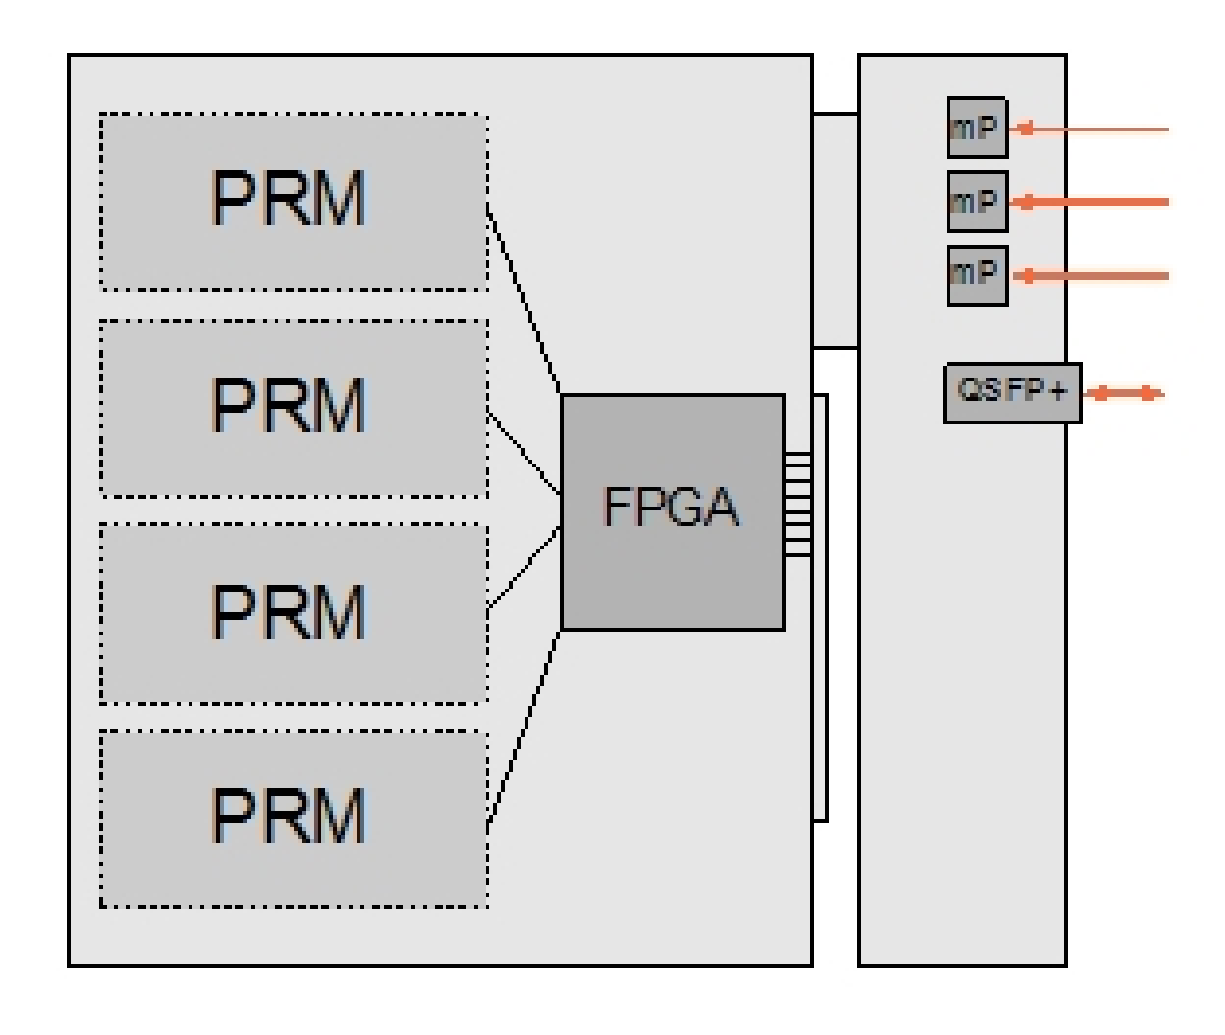
\includegraphics[width=0.45\columnwidth]{Plots/CombBlade.eps}
\caption{Combined blade design}
\label{fig:CombBlade}
\end{figure}


\noindent A tower shelf would then consist of 10 of Processor blades, one Gateway blade (for data sharing), and one Collector blade (for tracks found).  Backplane transfers are described in a series of fully pipelined sequences shown in Figure~\ref{fig:BackPlaneTr}.

\begin{figure}[ht!]
\centering
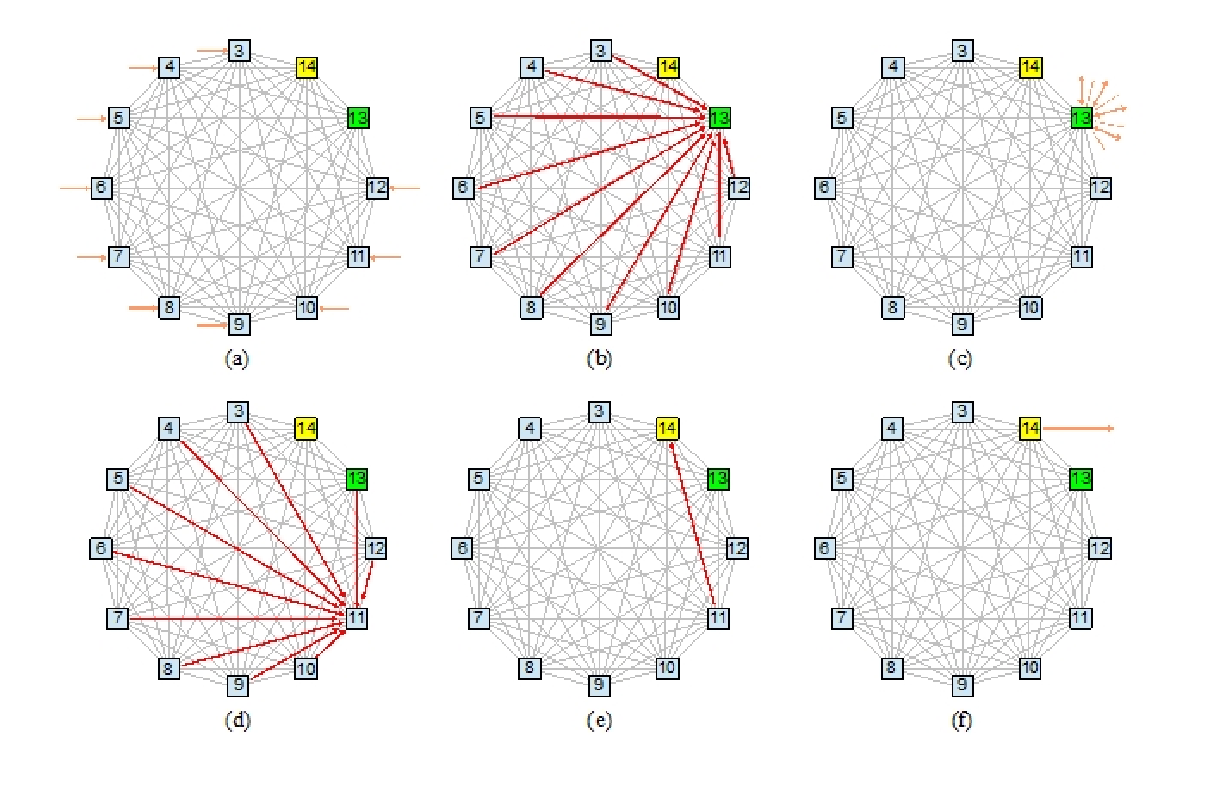
\includegraphics[width=0.85\columnwidth]{Plots/BackPlaneTr.eps}
\caption{Backplane transfers sequences using the combined blade design. First, the input fibers are received on the Processor blades (a).  Each Processor blade then transfers a portion of the input data to the Gateway blade (b), where it is exchanged with neighboring towers over fiber links (c).  The Processor blades and Gateway blade transfer the event (including neighbor data) to the target Processor blade in a time multiplexed, round robin scheme (d).   Results from the Processor blades are then transferred to the Collector blade (e) for any final formatting and processing before transmission downstream (f).}
\label{fig:BackPlaneTr}
\end{figure}
 

\noindent This processor architecture uses every channel in the full mesh backplane.  By using the full mesh fabric more effectively we are able to decrease the channel bandwidth requirement from 20 Gbps down to 6 Gbps with no significant latency increase. 

\noindent In summary, the architecture proposed here for the CMS L1 tracking trigger system is based on ATCA with full-mesh backplane. The large inter-board communication bandwidth provided by the full-mesh backplane is used to time multiplex the high volume (~ 50 Tbps) of incoming data in such a way that the I/O bandwidth demands are manageable at the board and chip level, making it possible for an early technical demonstration with existing technology. The resulting architecture is scalable, flexible and open. For example, it allows different pattern recognition architectures and algorithms to be explored and compared within the same platform. Also, given that AMC specifications are designed to work with both ATCA and MicroTCA, this architecture allows a natural long-term integration of TK-DAQ (AMC card based) and TK-TRIG (ATCA based).  In Section 3, we will describe the concept of how to build a vertical slice system demonstration based on this flexible architecture. 























\clearpage
